\documentclass{article}
\usepackage{tkz-tab}
\usepackage{amsmath} 
\usepackage{geometry}
\usepackage{indentfirst}
\setlength{\parindent}{0cm} % Retrait du paragraphe
\geometry{
    left=1cm }
\begin{document}
\underline{Tableau de variation de $f(x)$}\\
                   
$f(x)=\log{\left(x \right)}$\\
$f'(x)=\frac{1}{x}$\\

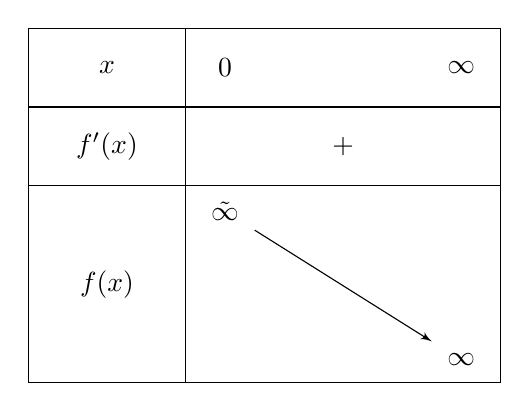
\begin{tikzpicture}
\tkzTabInit[espcl=3]{$x$ / 1 , $f'(x)$ / 1, $f(x)$/2.5}
{$0$,$\infty$}
\tkzTabLine{,+}
\tkzTabVar{+/$\tilde{\infty}$,-/$\infty$}

\end{tikzpicture}
\end{document}